\addcontentsline{toc}{chapter}{Занятие 6. Стохастическая непрерывность случайного процесса.
                                Существование непрерывной модификации}
\chapter*{Занятие 6. Стохастическая непрерывность случайного процесса.
          Существование непрерывной модификации}

\addcontentsline{toc}{section}{Контрольные вопросы и задания}
\section*{Контрольные вопросы и задания}

\subsubsection*{Приведите опредедение стохастически непрерывного процесса.}

Стохастически непрерывный процесс:
$ \xi \left( t \right) \overset{P} \xi \left( t_0 \right), \, t \to t_0$.

Это означает, что
$ \forall \varepsilon > 0 \qquad
  P \left( \left| \xi \left( t \right) - \xi \left( t_0 \right) \right| > \varepsilon \right) \to 0,
  \, t \to t_0$.

\subsubsection*{Сформулируйте достаточное условие существования непрерывной модификации случайного
                процесса.}

Пусть $ \xi \left( t \right), \, t \in \left[ 0, 1 \right] $ удовлетворяет условию
$$ \exists \alpha, \beta, C > 0: \qquad
  \forall t_1, t_2 \in \left[ 0, 1 \right] \qquad
  M \left| \xi \left( t_1 \right) =
  \xi \left( t_2 \right) \right|^{ \alpha } \leq C \left| t_1 - t_2 \right|^{1 + \beta }.$$
Тогда $ \xi $ имеет непрерывную модификацию.

\addcontentsline{toc}{section}{Аудиторные задачи}
\section*{Аудиторные задачи}

\subsubsection*{6.4}

\textit{Задание.}
Пусть $ \left\{ \xi \left( t \right), \, t \in \left[ 0, 1 \right] \right\} $ ---
случайный процесс, все значения которого являются независимыми и имеют одинаковое невырожденное
распределение.
Докажите, что этот процесс не является стохастически непрерывным ни в какой точке.

\textit{Решение.}
Распределения невырождены в том смысле, что это не константа (рис. \ref{fig:64}).

\begin{figure}[h!]
  \centering
  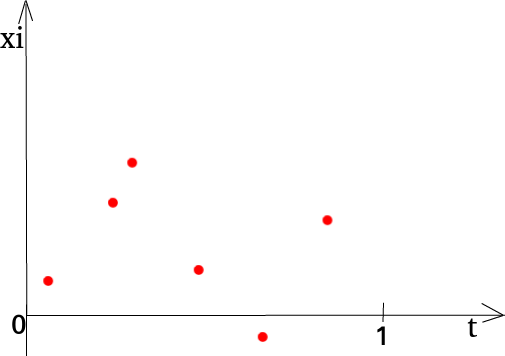
\includegraphics[width=.4\textwidth]{./pictures/6_4.png}
  \caption{График функции $ \xi \left( t \right) $}
  \label{fig:64}
\end{figure}

Стохастическая непрерывность означает, что вероятность
$$P \left\{ \left| \xi \left( s \right) - \xi \left( t \right) \right| > \varepsilon \right\} \to
  0.$$

Предположим, что распределение равномерное на отрезке $ \left[ 0, 1 \right] $.

Тогда такая вероятность равна
$$P \left\{ \left| \xi \left( s \right) - \xi \left( t \right) \right| > \varepsilon \right\} =
  \left( 1 - \varepsilon \right)^2 \not \to
  0, \,
  t \to s$$
(рис. \ref{fig:641}).

\begin{figure}[h!]
  \centering
  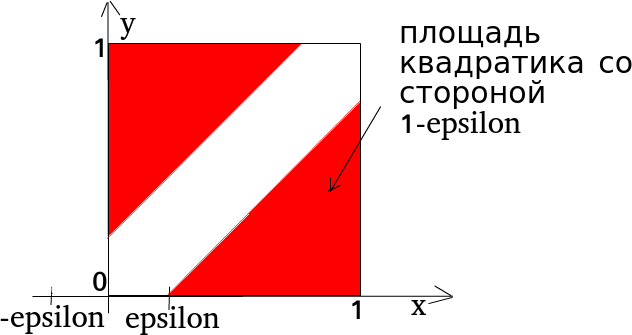
\includegraphics[width=.4\textwidth]{./pictures/6_4_1.png}
  \caption{Площадь квадратика со стороной $1 - \varepsilon$}
  \label{fig:641}
\end{figure}

Для такого процесса вероятность --- это постоянная и она не может стремиться к нулю.

\subsubsection*{6.5}

\textit{Задание.}
Пусть $X = \left\{ X \left( t \right), \, t \in T \right\} $ ---
стохастически непрерывный случайный процесс.
Докажите, что для произвольной непрерывной ограниченной функции $g$ функция
$M \left[ g \left( X \left( t \right) \right) \right] $ является непрерывной по $t$.

\textit{Решение.}
Нужно проверить, что если $t \to t_0$, то
$$M \left[ g \left( X \left( t \right) \right) \right] \to
  M \left[ g \left( X \left( t_0 \right) \right) \right].$$

Знаем, что если $t \to t_0$, то
$$X \left( t \right) \overset{P}{ \to }
  X \left( t_0 \right).$$
Следовательно, есть слабая сходимость.
Она как раз и означает, что такие математические ожидания должны сходиться.

\subsubsection*{6.7}

\textit{Задание.}
Пусть $ \left\{ \xi \left( t \right), \, t \in \left[ a, b \right] \right\} $ ---
стохастически непрерывный процесс, а $f$ --- неслучайная функция,
определённая на $ \left[ a, b \right] $.
Докажите, что случайный процесс
$ \eta \left( t \right) =
  \xi \left( t \right) + f \left( t \right), \, t \in \left[ a, b \right] $
является стохастически непрерывным в тех и только тех точках отрезка $ \left[ a, b \right] $,
где является непрерывной функция $f$.

\textit{Решение.}
Нужно доказывать в обе стороны.

Сначала предположим, что $f$ --- непрерывная.
Пусть $f$ --- непрерывная в точке $t_0$.
Будем сейчас проверять, что сумма стохастически непрерывна.

Если $ \xi \left( t \right) $ --- стохастически непрерывна, то
$$ \xi \left( t \right) \overset{P}{ \to }
  \xi \left( t_0 \right)$$
при $t \to t_0$.

Сходимость по вероятности сохраняется при непрерывных операциях.
Сумма --- непрерывная операция.

Знаем, что $f$ --- непрерывна, то есть если $t \to t_0$,
то $f \left( t \right) \to f \left( t_0 \right) $.
От $ \omega $ тут зависимости нет.
Эту сходимость можно интерпретировать как сходимость почти наверное, следовательно,
$$f \left( t \right) \overset{P}{ \to }
  f \left( t_0 \right).$$

Значит и сумма будет сходиться.
Значит, отсюда следует, что $ \eta $ --- стохастически непрерывен.

Теперь предоложим, что вся сумма стохастически непрерывна.

Пусть $ \eta $ --- стохастически непрерывен в $t_0$.
Это значит, что
$$ \eta \left( t \right) \overset{P}{ \to } \eta \left( t_0 \right), \,
  t \to t_0.$$

Для $ \eta $ и $ \xi $ мы знаем, что есть сходимость по вероятности.
Надо взять разность.
Разность --- это $f$, то есть
$$ \begin{cases}
    \xi \left( t \right) + f \left( t \right) \overset{P}{ \to }
    \xi \left( t_0 \right) + f \left( t_0 \right), \\
    \xi \left( t \right) \overset{P}{ \to } \xi \left( t_0 \right).
  \end{cases}$$

Вычтем из первого второе
$$f \left( t \right) \overset{P}{ \to }
  f \left( t_0 \right).$$
Нужно проверить, что для неслучайной функции сходимость по вероятности и просто сходимость ---
одно и то же.
Сходимость по вероятности:
$ \forall \varepsilon > 0 \qquad
  P \left\{ \left| f \left( t \right) - f \left( t_0 \right) \right| > \varepsilon \right\} \to 0,
  \, t \to t_0$.
Это есть.
Просто сходимость: $ \forall \varepsilon > 0 \, \exists \delta > 0$,
чтобы выполнялось соотношение
$ \left| f \left( t \right) - f \left( t_0 \right) \right| <
  \varepsilon $
при $ \left| t - t_0 \right| < \delta $.
Это нужно проверить.

$ \forall \varepsilon > 0 \, \forall \alpha > 0 \, \exists \delta > 0 \qquad
  P \left\{ \left| f \left( t \right) - f \left( t_0 \right) \right| > \varepsilon \right\} <
  \alpha $
при $ \left| t - t_0 \right| < \delta $.

Функция $f$ --- неслучайная функция, то есть событие неслучайно.
Его вероятность равна или нулю, или единице.
Если $ \alpha > 1$, то вероятность равна нулю.
Значит, $ \left| f \left( t \right) - f \left( t_0 \right) \right| < \varepsilon $ при
$ \left| t - t_0 \right| <
  \delta $.
То есть $ \alpha < 1$.

Тогда
$P \left\{ \left| f \left( t \right) - f \left( t_0 \right) \right| > \varepsilon \right\} =
  0$.
Из этого следует, что при $ \left| t - t_0 \right| < \delta $ выполняется дополнение
$ \left| f \left( t \right) - f \left( t_0 \right) \right| \leq
  \varepsilon $.
Это и значит непрерывность в точке $t_0$.
Таким образом, для неслучайных величин все сходимости равносильны.

\subsubsection*{6.8}

\textit{Задание.}
Пусть $ \left\{ W \left( t \right), \, t \geq 0 \right\} $ --- винеровский процесс.
Докажите, что для произвольного $A > 0$
$$P \left\{
    \sum \limits_{i = 0}^{n - 1}
      \left| W \left( \frac{i + 1}{n} \right) - W \left( \frac{i}{n} \right) \right| > A
  \right\} \to
  1, \,
  n \to \infty.$$

\textit{Решение.}
Приращения --- нормальные независимые величины
$$W \left( \frac{i + 1}{n} \right) - W \left( \frac{i}{n} \right) \sim
  N \left( 0, \frac{1}{n} \right).$$

Сумма одинаково распределённых случайных величин
$$ \frac{1}{n} \sum \limits_{i = 1}^{n - 1}
    \left| W \left( \frac{i + 1}{n} \right) - W \left( \frac{1}{n} \right) \right| \cdot
  \sqrt{n} \overset{a.s.}{ \to }
  M \left| W \left( 1 \right) \right|, \,
  n \to \infty $$
по усиленному закону больших чисел, так как
$$ \sqrt{n} \left[ W \left( \frac{i + 1}{n} \right) - W \left( \frac{i}{n} \right) \right] \sim
  N \left( 0, 1 \right).$$

Тогда вероятность
$$P \left\{
    \sum \limits_{i = 0}^{n - 1}
      \left| W \left( \frac{i + 1}{n} \right) - W \left( \frac{i}{n} \right) \right| \cdot
    \frac{ \sqrt{n}}{n} \cdot \frac{n}{ \sqrt{n}} > A \right\} =
  P \left\{ M \left| W \left( 1 \right) \right| > 0 \right\} =
  1.$$

\subsubsection*{6.9}

\textit{Задание.}
Пусть $ \left\{ X \left( t \right), \, t \in T \right\} $ --- случайный процесс такой, что
$$MX \left( t \right) = 0, \,
  MX^2 \left( t \right) = 1$$
для произвольного $t \in T$.
\begin{enumerate}[label=\alph*)]
  \item Докажите, что $ \left| MX \left( t \right) X \left( t + h \right) \right| \leq 1$
  для произвольного $h > 0$ и произвольного $t \in \left[ 0, T - h \right] $.
  \item Допустим, что для некоторых $ \lambda < \infty, \, p > 1$ и $h_0 > 0$
  $$M \left[ X \left( t \right) X \left( t + h \right) \right] \geq
    1 - \lambda h^p$$
  для произвольного $h \in \left( 0, h_0 \right] $.
  Докажите, что $ \left\{ X \left( t \right), \, t \in T \right\} $ имеет непрерывную модификацию.
\end{enumerate}

\textit{Решение.}
\begin{enumerate}[label=\alph*)]
  \item Пусть $X \left( t \right) = \xi $ и $X \left( t + h \right) = \eta $.
  Тогда
  $$ \left| M \xi \eta \right| \leq
    M \left| \xi \eta \right| \leq
    \left( M \left| \xi \right|^p \right)^{ \frac{1}{p}}
    \left( M \left| \eta \right|^q \right)^{ \frac{1}{q}},$$
  где
  $$ \frac{1}{p} + \frac{1}{q} =
    1$$
  (неравенство Гёльдера).
  Возьмём $p = q = 2$.

  Получаем неравенство Коши-Буняковского
  $$M \left[ X \left( t \right) X \left( t + h \right) \right] \leq
    \left\{ M \left| X \left( t \right) \right|^2 \right\}^{ \frac{1}{2}}
    \left\{ M \left| X \left( t + h \right) \right|^2 \right\}^{ \frac{1}{2}} =
    1 \cdot 1 =
    1.$$
  \item Будем пользоваться достаточным условием Колмогорова
  $$ \exists \alpha, \beta, C > 0 \, : \,
    \forall t_1, t_2 \in \left[ 0, 1 \right] \qquad
    M \left| \xi \left( t_1 \right) - \xi \left( t_2 \right) \right|^{ \alpha } \leq
    C \left| t_1 - t_2 \right|^{1 - \beta }.$$
  Тогда у процесса будут непрерывные модификации.
  Нужно оценить
  $$M \left| X \left( t + h \right) - X \left( t \right) \right|^2 =
    M\left[X^2\left(t+h\right)-2X\left(t+h\right)X\left(t\right)+X^2\left(t\right)\right] =$$
  Воспользуемся линейностью математического ожидания
  $$= MX^2 \left( t + h \right) - 2M \left[  X \left( t + h \right) X \left( t \right) \right] +
    MX^2 \left( t \right).$$
  Здесь первое и последнее слагаемые равны единице, а второе не меньше $1 - \lambda h^p$.
  Тогда
  $$MX^2 \left( t + h \right) - 2M \left[  X \left( t + h \right) X \left( t \right) \right] +
    MX^2 \left( t \right) \geq
    2 - 2 \left( 1 - \lambda h^p \right) =
    2 \lambda h^p,$$
  где $2 \lambda = const, \, p = 1 + \beta $.

  Теорема Колмогорова работает с $ \alpha = 2, \, C = 2 \lambda $ и $ \beta = p - 1$.

  Значит, такой процесс имеет непрерывные модификации.
\end{enumerate}

\addcontentsline{toc}{section}{Домашнее задание}
\section*{Домашнее задание}

\subsubsection*{6.17}

\textit{Задание.}
Пусть все значения процесса $ \left\{ X \left( t \right), \, t \in \mathbb{R}^+ \right\} $
являются независимыми и равномерно распределёнными на $ \left[ 0, 1 \right] $.
Выясните, имеет ли этот процесс непрерывную модификацию.

\textit{Решение.}
Из задачи 6.4 $X \left( t \right) $ не стохастически непрерывен в каждой точке.

Стохастическая непрерывность означает,
что $X \left( t \right) \overset{P}{ \to } X \left( t_0 \right) $ при $t \to t_0$.

Пусть процесс $X \left( t \right) $ имеет непрерывную модификацию.
Тогда
$$ \begin{cases}
    X \left( t \right) = \tilde{X} \left( t \right) \, a.s., \\
    \tilde{X} \left( t \right) \to \tilde{X} \left( t_0 \right), \, t \to t_0, \\
    X \left( t_0 \right) = \hat{X} \left( t_0 \right) \, a.s.
  \end{cases} \Rightarrow X \left( t \right) \to X \left( t_0 \right) \, a.s.,$$
то есть процесс $X \left( t \right) $ стохастически непрерывен --- противоречие с условием.
Значит, $X \left( t \right) $ не имеет непрерывной модификации.

\subsubsection*{6.18}

\textit{Задание.}
Пусть $X = \left\{ X \left( t \right), \, t \in \mathbb{R}^+ \right\} $ ---
гауссовский процесс с нулевым математическим ожиданием и ковариационной функцией
$K \left( t, s \right) $, которая равна
\begin{enumerate}[label=\alph*)]
  \item $e^{-\left| t - s \right| }$,
  \item $ \left( t^{ \alpha } + s^{ \alpha } - \left| t - s \right|^{ \alpha } \right) / 2, \,
    \alpha \in \left( 0, 2 \right] $.
\end{enumerate}
Докажите, что $X$ имеет непрерывную модификацию.

\textit{Решение.}
Нам нужно доказать, что существуют такие константы
$$ \alpha > 0, \,
  \beta > 0, \,
  C > 0,$$
что
$M \left| X \left( t + h \right) - X \left( t \right) \right|^{ \alpha} \leq
  C \left| h \right|^{1 + \beta }$
для произвольных $t, \, t + h \in \mathbb{R}^+, \, h > 0$.

Поскольку процесс $X$ является гауссовским, то для произвольных
$$t, \, t + h \in \mathbb{R}^+$$
вектор $ \left( X \left( t \right), X \left( t + h \right) \right) $ является гауссовским.
Поэтому случайная величина $X \left( t + h \right) - X \left( t \right) $,
как линейная комбинация компонент гауссовского вектора, имеет нормальное распределение.
Найдём параметры этого распределения.
Имеем
$M \left[ X \left( t + h \right) - X \left( t \right) \right] =
  MX \left( t + h \right) - MX \left( t \right) =
  0$,
\begin{enumerate}[label=\alph*)]
  \item $D \left[ X \left( t + h \right) - X \left( t \right) \right] =
    M \left[ X \left( t + h \right) - X \left( t \right) \right]^2.$
  Раскроем квадрат
  $$M \left[ X \left( t + h \right) - X \left( t \right) \right]^2 =
    K \left( t + h, t + h \right) - 2K \left( t + h, t \right) + K \left( t, t \right) =$$
  Подставим выражения для ковариационной функции
  $$= e^{-\left| t + h - t - h \right| } - 2e^{-\left| t + h - t \right| } +
    e^{-\left| t - t \right| } =
    1 - 2e^{-\left| h \right| } + 1 =
    2 - 2e^{-h}.$$

  Тогда любой чётный момент случайной величины $X \left( t + h \right) - X \left( t \right) $ равен
  $M \left[ X \left( t + h \right) - X \left( t \right) \right]^{2n} =
    \left( 2n - 1 \right)!! \left( 2 - 2e^{-h} \right)^n$.

  Поскольку $1 - e^{-h} \leq h$ для $h > 0$,
  то $M \left[ X \left( t + h \right) - X \left( t \right) \right]^4 \leq 12h^2$ и, значит,
  достаточное условие Колмогорова существования непрерывной модификации выполняется при
  $ \alpha = 4, \,
    \beta = 1, \,
    C = 12$.
  \item Имеем
  $$D \left[ X \left( t + h \right) - X \left( t \right) \right] =
    M \left[ X \left( t + h \right) - X \left( t \right) \right]^2 =$$
  Раскроем квадрат
  \begin{gather*}
    = K \left( t + h, t + h \right) - 2K \left( t + h, t \right) + K \left( t, t \right) = \\
    = \frac{\left(t+h\right)^{\alpha}+\left(t+h\right)^{\alpha}-\left|t+h-t-h\right|^{\alpha}}{2}- \\
    - 2\cdot\frac{\left(t+h\right)^{\alpha}+t^{\alpha}-\left|t+h-t\right|^{\alpha}}{2} +
    \frac{t^{ \alpha } + t^{ \alpha } - \left| t - t \right|^{ \alpha }}{2} = \\
    = \left( t + h \right)^{ \alpha } - \left( t + h \right)^{ \alpha } - t^{ \alpha } -
    h^{ \alpha } + t^{ \alpha } =
    -h^{ \alpha }.
  \end{gather*}

  Тогда любой чётный момент случайной величины $X \left( t + h \right) - X \left( t \right) $ равен
  $M \left[ X \left( t + h \right) - X \left( t \right) \right]^{2n} =
    \left( 2n - 1 \right)!! \left( -h^{ \alpha } \right)^n$.

  В частности,
  $M \left[ X \left( t + h \right) - X \left( t \right) \right]^2 =
    3!! \left( -h^{ \alpha } \right) =
    3h^{ \alpha }$
  и, значит, достаточное условие Колмогорова существования непрерывной модификации выполняется при
  $ \alpha = 2, \,
    \beta = \alpha - 1 = 2 - 1 = 1, \,
    C = 3$.
\end{enumerate}

\subsubsection*{6.19}

\textit{Задание.}
Для процесса Пуассона найдите предел с вероятностью единица последовательности случайных величин
$$ \sum \limits_{i = 0}^{n - 1} \left( N \left( t_{i + 1} \right) - N \left( t_i \right) \right)^2$$
при $ \max \left( t_{i + 1} - t_i \right) \to 0$, где $0 = t_0 < t_1 < \dotsc < t_n = 1$ ---
разбитие отрезка $ \left[ 0, 1 \right] $.

\textit{Решение.}
$$P \left\{
    \sum \limits_{i = 0}^{n - 1} \left[ N \left( t_{i + 1} \right) - N \left( t_i \right) \right]^2 >
    \varepsilon \right\} \leq
  \frac{M\sum\limits_{i=0}^{n-1}\left[N\left(t_{i+1}\right)-N\left(t_i\right)\right]^2}{\varepsilon} =$$
Пользуемся независимостью приращений
$$=\frac{\sum\limits_{i=0}^{n-1}M\left[N\left(t_{i+1}\right)-N\left(t_i\right)\right]^2}{\varepsilon} =$$
Пользуемся однородностью приращений
$$= \frac{ \sum \limits_{i = 0}^{n - 1} MN^2 \left( t_{i + 1} - t_i \right) }{ \varepsilon } =
  \frac{1}{ \varepsilon }
  \sum \limits_{i = 0}^{n - 1}
    \left[ DN \left( t_{i + 1} - t_i \right) + M^2 N \left( t_{i + 1} - t_i \right) \right] =$$
Пусть случайная величина $X \left( t \right) $ с распределением Пуассона имеет параметр $ \lambda $.
Тогда
$$= \frac{1}{ \varepsilon }
  \sum \limits_{i = 0}^{n - 1} \left[
  \lambda \left( t_{i + 1} - t_i \right) + \lambda^2 \left( t_{i + 1} - t_i \right)^2 \right] =
  \frac{1}{ \varepsilon }
  \sum \limits_{i = 0}^{n - 1}
    \lambda \left( t_{i + 1} - t_i \right)
    \left[ 1 + \lambda \left( t_{i + 1} - t_i \right) \right] \leq$$
Оценим сумму максимумом
$$\leq \frac{n}{ \varepsilon } \cdot \left\{
    \lambda \max \left( t_{i + 1} - t_i \right)
    \left[ 1 + \lambda \max \left( t_{i + 1} - t_i \right) \right] \right\} \to
  0$$
при $ \max \left( t_{i + 1} - t_i \right) \to 0$, следовательно, предел по вероятности равен нулю.
